\documentclass[11pt]{article}
\usepackage[margin=0.85in, top=0.7in, bottom=0.7in]{geometry}
\usepackage{enumitem}
\usepackage{graphicx}
\usepackage{booktabs}
\usepackage{caption}
\usepackage{subcaption}
\usepackage{amsmath}
\usepackage{hyperref}
\usepackage{xcolor}

\newcommand{\todo}[1]{\textcolor{red}{\textbf{[TODO: #1]}}}

% ─────────────────────────────────────────────────────────────────────────────
\begin{document}

% ── Title Page ───────────────────────────────────────────────────────────────
\begin{titlepage}
  \centering
  \vspace*{1.5cm}
  {\large Neural Networks\\[0.4em]
          COMP/EECE 7/8740 \\[2.5cm]}
  {\LARGE\bfseries Final Project Report\\[0.6em]
   \large Procedural Geographic Map Generation\\[0.3em]
   via Generative Adversarial Networks\\[2.5cm]}
  {\large
   \begin{tabular}{rl}
     Name: & Jace King \\[0.5em]
     ID:   & U00969076  \\
   \end{tabular}\\[2.5cm]}
  {\large \today}
  \vfill
\end{titlepage}

% ── Abstract ─────────────────────────────────────────────────────────────────
\newpage
\begin{abstract}
\noindent
We train Wasserstein GANs with gradient penalty (WGAN-GP) and a DCGAN-style
convolutional architecture to reproduce the distribution of $128{\times}128$ RGB
terrain maps generated by layered simplex/Perlin noise. Seven generators, one
per hand-tuned noise preset, were trained for 50 epochs each on 3{,}000 images
per class. The unconditional models recover the macro-scale land/water layout
for several presets but fail to reproduce the discrete six-tier terrain palette
and exhibit single-feature mode collapse on three of the seven. A conditional
variant (cDCGAN) over all seven presets simultaneously was attempted but did
not finish within the available compute budget (epoch 14/50 at
$\sim$76\,min/epoch on CPU). We report training curves, qualitative samples, and quantitative evaluation of
all seven generators against the held-out test set using FID, radial
power-spectrum slope, palette color fidelity, and A*-based navigability
metrics. The trained preset\_01 generator is integrated into a real-time A*
navigation game via a NumPy-only inference path with snap-to-palette
post-processing.
\end{abstract}

% ─────────────────────────────────────────────────────────────────────────────
\section{Introduction}
Procedural content generation in games has historically relied on hand-tuned
noise functions, where a small parameter vector controls the visual character
of an output. A generative model that learns this distribution end-to-end
offers two practical advantages: (i)~a single trained model can replace the
parameter-tuning workflow with a latent-space sampling interface, and
(ii)~a conditional model can interpolate between or smoothly mix the
qualitative ``flavors'' of distinct presets, which a hand-coded generator
cannot do without explicit blending logic.

We restrict the problem to a tractable supervised setting: the data
distribution itself is fixed and known (layered simplex/Perlin noise with a
piecewise-constant terrain palette), the resolution is moderate
($128{\times}128$), and the seven terrain types are well separated in
parameter space. Our goal is to train a GAN that reproduces this distribution
well enough for its output to be used as drop-in terrain maps in a simple
navigation game, and to evaluate the degree to which the learned distribution
matches the real one using both visual and quantitative criteria.

% ─────────────────────────────────────────────────────────────────────────────
\section{Methodology}
We frame terrain generation as an unconditional generative modeling problem:
train a generator $G$ to map Gaussian noise $\mathbf{z}$ to synthetic terrain
images whose distribution is indistinguishable from layered Perlin-noise maps.
For each of the seven hand-tuned noise presets we train a separate
unconditional model; a seventh, conditional model is trained jointly over all
presets. We use the Wasserstein GAN with gradient penalty (WGAN-GP)
\cite{gulrajani2017improved} rather than vanilla DCGAN
\cite{radford2016dcgan} because of its superior training stability and
interpretable critic loss.

\subsection{Loss Function}
We use the WGAN-GP objective \cite{gulrajani2017improved}:
\begin{align*}
\mathcal{L}_D &= \mathbb{E}[D(G(\mathbf{z}))] - \mathbb{E}[D(\mathbf{x})]
              + \lambda \,\mathbb{E}\big[(\|\nabla_{\hat{\mathbf{x}}}
                     D(\hat{\mathbf{x}})\|_2 - 1)^2\big], \\
\mathcal{L}_G &= -\mathbb{E}[D(G(\mathbf{z}))],
\end{align*}
with $\hat{\mathbf{x}} = \alpha \mathbf{x} + (1-\alpha) G(\mathbf{z})$,
$\alpha \sim \mathrm{Uniform}[0,1]$, and $\lambda = 10$. We run
$n_{\text{disc}} = 5$ critic updates per generator update.

\subsection{Optimization}
Adam with $\eta = 2{\times}10^{-4}$, $\beta_1 = 0.5$, $\beta_2 = 0.999$ for
both networks. Batch size 64, seed 42 for the data shuffle and the fixed
evaluation $\mathbf{z}$. The original WGAN-GP paper recommends
$\beta_2 = 0.9$; we used the Adam default of $0.999$ and observed no
divergence in any of the eight runs, but a re-run with $\beta_2 = 0.9$ would
be the more conservative choice.

\subsection{Compute}
Training was performed on a SLURM cluster, one node per preset, 16 CPUs and
32\,GB RAM per task, no GPU available
(\texttt{tf.config.list\_physical\_devices('GPU')} returned \texttt{[]}).
Per-epoch wall time averaged $\sim$580--700\,s ($\sim$10--12\,min) for the
unconditional models and $\sim$4{,}600\,s ($\sim$76\,min) for the conditional
model; total wall time was $\sim$8--10\,h per unconditional run.

% ─────────────────────────────────────────────────────────────────────────────
\section{Model Description}
Following DCGAN conventions \cite{radford2016dcgan}, the generator $G$ maps a
100-dimensional latent vector $\mathbf{z} \sim \mathcal{N}(0,I)$ to a
$128{\times}128{\times}3$ image with $\tanh$ output. The discriminator
(critic) $D$ maps an image to an unbounded scalar.

\subsection{Generator (4.83\,M params)}
$\mathbf{z} \in \mathbb{R}^{100} \to \mathrm{Dense}(8{\cdot}8{\cdot}512) \to
\mathrm{Reshape}(8,8,512) \to \mathrm{BN} \to \mathrm{LReLU}(0.2)$, then three
upsampling blocks
$$\big[\mathrm{UpSample2x} \to \mathrm{Conv2D}(3{\times}3) \to \mathrm{BN}
       \to \mathrm{LReLU}(0.2)\big]$$
with channel widths $\{256, 128, 64\}$ ($8{\to}16{\to}32{\to}64$), followed by
a final $\mathrm{UpSample2x} \to \mathrm{Conv2D}(3{\times}3, \tanh)$ to
$3$ channels at $128{\times}128$.

\subsection{Critic (2.79\,M params)}
Four strided conv blocks $\mathrm{Conv2D}(4{\times}4,\,\text{stride}\,2)
\to \mathrm{LReLU}(0.2)$ with widths $\{64, 128, 256, 512\}$
($128{\to}64{\to}32{\to}16{\to}8$), then $\mathrm{Flatten} \to
\mathrm{Dense}(1)$. We use \emph{no normalization} in the critic: BatchNorm
couples samples within a minibatch and is incompatible with the per-sample
gradient penalty.

\subsection{Conditional Variant (cDCGAN)}
For the cDCGAN, a 7-dim one-hot label is concatenated to $\mathbf{z}$ before
the generator's first Dense layer, and to the critic's flattened feature
vector before its final Dense layer. All other architectural choices are
unchanged; the conditioning adds $\sim$5\% to the parameter count.

% ─────────────────────────────────────────────────────────────────────────────
\section{Experiments and Results}

\subsection{Database}
The training dataset consists of 21{,}000 images: 3{,}000 per preset for seven
presets. Each image is $128{\times}128$ RGB, $\mathtt{uint8}$. A held-out test
set of 1{,}400 images (200 per preset) is reserved for evaluation. All images
are produced by \texttt{generate\_dataset.py} from layered simplex noise via
\texttt{noise2array}.

\paragraph{Presets.}
Each preset fixes a base $(\text{depth},\,\text{scale},\,\text{factor},\,
\text{persistence})$ tuple. To prevent the GAN from memorizing a small
template set, every image samples (i)~a random spatial offset
$(x_0,y_0) \in [0,9999]^2$ in noise space and (ii)~multiplicative jitter on
the parameters: scale $\pm 15\%$, persistence $\pm 10\%$, factor $\pm 10\%$.

\paragraph{Color palette.}
The continuous noise field $n \in \mathbb{R}$ is normalized to $[0,1]$ and
quantized through six fixed thresholds into the categorical palette
\{deep water, shallow water, sand, plains, mountains, mountain tops\}.
This piecewise-constant mapping is the most challenging structural feature
of the data for a tanh-output convolutional generator to reproduce, as
discussed in Section~\ref{sec:discussion}.

\paragraph{Reference samples.}
Figure~\ref{fig:presets} shows one representative sample from each preset.

\begin{figure}[h]
  \centering
  \begin{subfigure}[t]{0.13\textwidth}\centering
    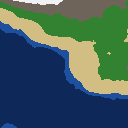
\includegraphics[width=\linewidth]{../presets/preset_01.png}\\\small preset\_01
  \end{subfigure}\hfill
  \begin{subfigure}[t]{0.13\textwidth}\centering
    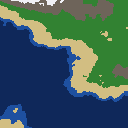
\includegraphics[width=\linewidth]{../presets/preset_02.png}\\\small preset\_02
  \end{subfigure}\hfill
  \begin{subfigure}[t]{0.13\textwidth}\centering
    
\includegraphics[width=\linewidth]{../presets/preset_03.png}\\\small preset\_03
  \end{subfigure}\hfill
  \begin{subfigure}[t]{0.13\textwidth}\centering
    
\includegraphics[width=\linewidth]{../presets/preset_04.png}\\\small preset\_04
  \end{subfigure}\hfill
  \begin{subfigure}[t]{0.13\textwidth}\centering
    
\includegraphics[width=\linewidth]{../presets/preset_05.png}\\\small preset\_05
  \end{subfigure}\hfill
  \begin{subfigure}[t]{0.13\textwidth}\centering
    
\includegraphics[width=\linewidth]{../presets/preset_06.png}\\\small preset\_06
  \end{subfigure}\hfill
  \begin{subfigure}[t]{0.13\textwidth}\centering
    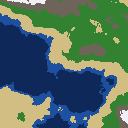
\includegraphics[width=\linewidth]{../presets/preset_07.png}\\\small preset\_07
  \end{subfigure}
  \caption{One representative real sample per preset. Note the categorical
           color palette and the highly preset-specific land/water ratios.}
  \label{fig:presets}
\end{figure}

% ─────────────────────────────────────────────────────────────────────────────
\subsection{Training and Testing Logs}

\subsubsection*{Training curves}
Figure~\ref{fig:loss} plots the per-epoch mean $\mathcal{L}_G$ and
$\mathcal{L}_D$ for each preset from \texttt{logs/dcgan\_preset\_*.csv},
rendered by \texttt{scripts/plot\_loss\_curves.py}.

\begin{figure}[h]
  \centering
  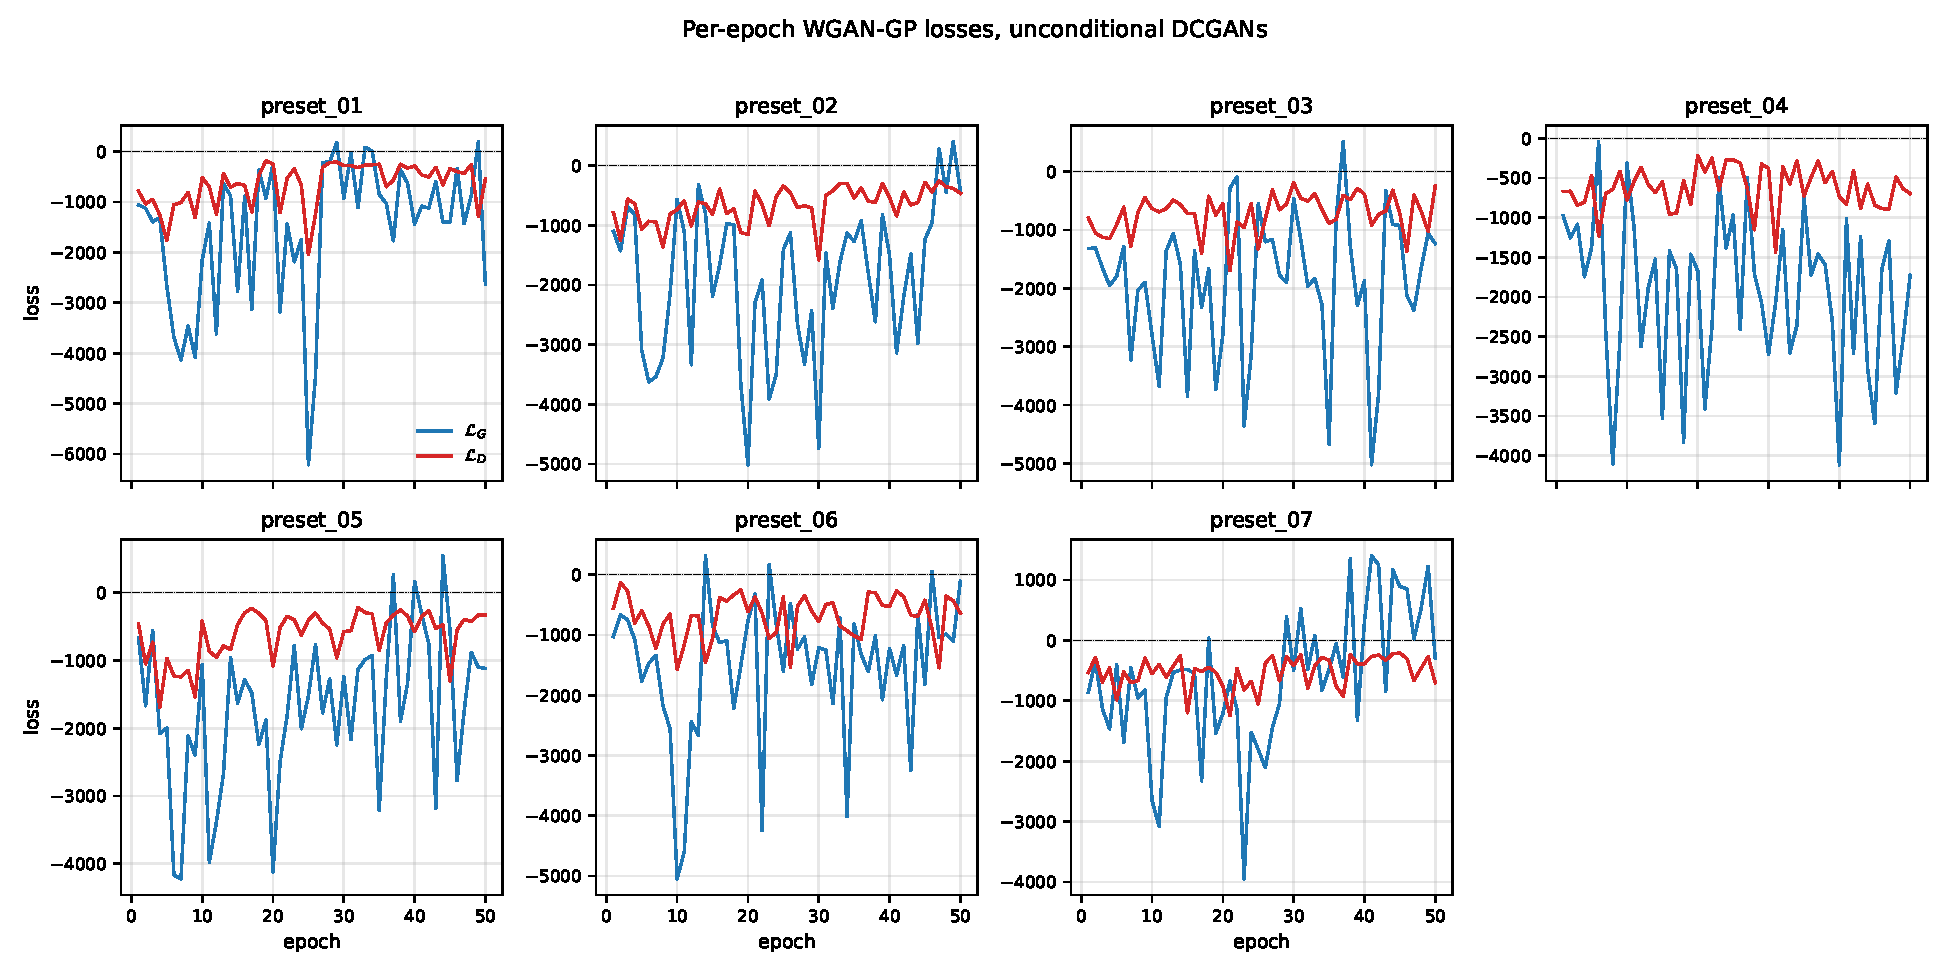
\includegraphics[width=0.95\textwidth]{../figures/loss_curves.pdf}
  \caption{Per-epoch generator and critic losses for each unconditional preset
           over 50 epochs of WGAN-GP training.}
  \label{fig:loss}
\end{figure}

The Wasserstein critic loss is unbounded by construction; large negative
values and substantial epoch-to-epoch variance are expected and do not by
themselves indicate failure. Across all seven presets the magnitude of both
$\mathcal{L}_G$ and $\mathcal{L}_D$ is large in the first $\sim$10 epochs
(reflecting an under-converged critic), then settles into an oscillating but
bounded regime for the rest of training. Final-epoch values for
$\mathcal{L}_G$ range from $\sim\!-2{,}600$ (preset\_01) to $\sim\!-110$
(preset\_06); these absolute values are not directly comparable across
presets because the critic for each model is calibrated to its own data
distribution. We do not observe the diverging-loss / saturated-output failure
mode characteristic of vanilla DCGAN; the gradient penalty appears to keep
the critic in the 1-Lipschitz neighborhood throughout.

\subsubsection*{Generated samples}
\label{sec:samples}
Figure~\ref{fig:samples} shows the final-epoch fixed-noise sample grid for
each preset. All seven grids use the same $\mathbf{z}$ seed
(\texttt{tf.random.normal((64, 100), seed=0)}), so within-grid variation
reflects sensitivity to $\mathbf{z}$ for that generator.

\begin{figure}[h]
  \centering
  \begin{subfigure}[t]{0.23\textwidth}\centering
    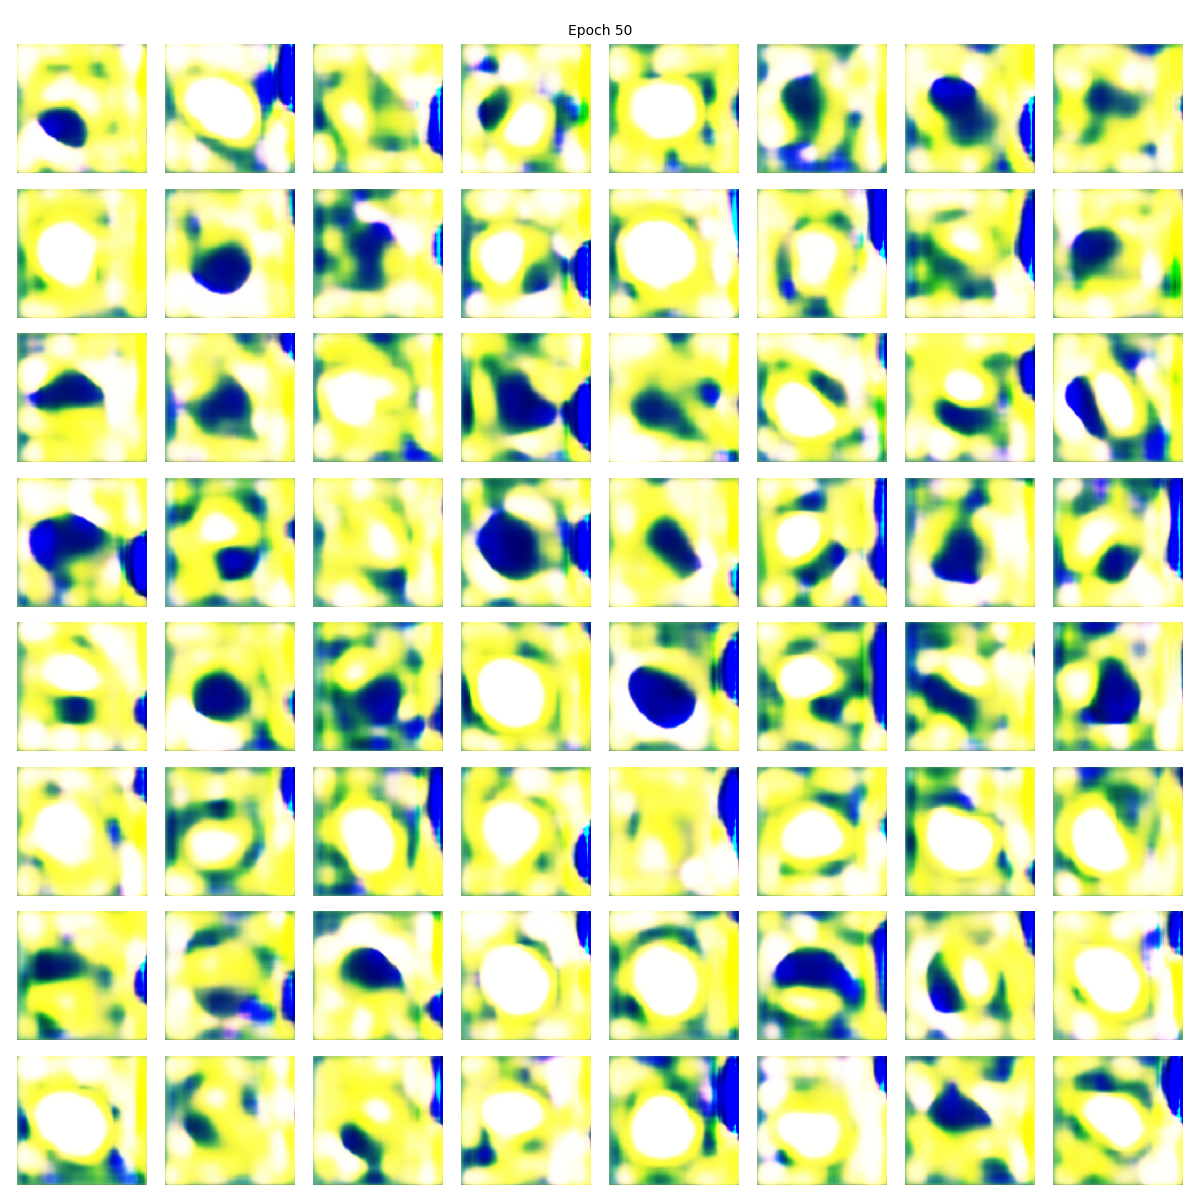
\includegraphics[width=\linewidth]{../samples/preset_01/final.png}
    \caption{preset\_01}
  \end{subfigure}\hfill
  \begin{subfigure}[t]{0.23\textwidth}\centering
    
\includegraphics[width=\linewidth]{../samples/preset_02/final.png}
    \caption{preset\_02}
  \end{subfigure}\hfill
  \begin{subfigure}[t]{0.23\textwidth}\centering
    
\includegraphics[width=\linewidth]{../samples/preset_03/final.png}
    \caption{preset\_03}
  \end{subfigure}\hfill
  \begin{subfigure}[t]{0.23\textwidth}\centering
    
\includegraphics[width=\linewidth]{../samples/preset_04/final.png}
    \caption{preset\_04}
  \end{subfigure}

  \vspace{0.5em}

  \begin{subfigure}[t]{0.23\textwidth}\centering
    
\includegraphics[width=\linewidth]{../samples/preset_05/final.png}
    \caption{preset\_05}
  \end{subfigure}\hfill
  \begin{subfigure}[t]{0.23\textwidth}\centering
    
\includegraphics[width=\linewidth]{../samples/preset_06/final.png}
    \caption{preset\_06}
  \end{subfigure}\hfill
  \begin{subfigure}[t]{0.23\textwidth}\centering
    
\includegraphics[width=\linewidth]{../samples/preset_07/final.png}
    \caption{preset\_07}
  \end{subfigure}
  \caption{Generator output at epoch 50, 64 samples per preset (same
           $\mathbf{z}$ seed across all presets).}
  \label{fig:samples}
\end{figure}

Figure~\ref{fig:snapped} shows the same generators' output after
snap-to-palette post-processing.

\begin{figure}[h]
  \centering
  \begin{subfigure}[t]{0.13\textwidth}\centering
    
\includegraphics[width=\linewidth]{../samples/snapped/preset_01.png}\\\small preset\_01
  \end{subfigure}\hfill
  \begin{subfigure}[t]{0.13\textwidth}\centering
    
\includegraphics[width=\linewidth]{../samples/snapped/preset_02.png}\\\small preset\_02
  \end{subfigure}\hfill
  \begin{subfigure}[t]{0.13\textwidth}\centering
    
\includegraphics[width=\linewidth]{../samples/snapped/preset_03.png}\\\small preset\_03
  \end{subfigure}\hfill
  \begin{subfigure}[t]{0.13\textwidth}\centering
    
\includegraphics[width=\linewidth]{../samples/snapped/preset_04.png}\\\small preset\_04
  \end{subfigure}\hfill
  \begin{subfigure}[t]{0.13\textwidth}\centering
    
\includegraphics[width=\linewidth]{../samples/snapped/preset_05.png}\\\small preset\_05
  \end{subfigure}\hfill
  \begin{subfigure}[t]{0.13\textwidth}\centering
    
\includegraphics[width=\linewidth]{../samples/snapped/preset_06.png}\\\small preset\_06
  \end{subfigure}\hfill
  \begin{subfigure}[t]{0.13\textwidth}\centering
    
\includegraphics[width=\linewidth]{../samples/snapped/preset_07.png}\\\small preset\_07
  \end{subfigure}
  \caption{Generator output after snap-to-palette post-processing
           ($4{\times}4$ samples per preset, same $\mathbf{z}$ seed as
           Figure~\ref{fig:samples}). Snapping maps each pixel to its
           nearest palette entry by Euclidean distance in RGB space,
           eliminating the smooth color interpolation and producing maps
           directly consumable by the game's speed-map lookup.}
  \label{fig:snapped}
\end{figure}

\subsubsection*{Quantitative evaluation}
\label{sec:eval}
Table~\ref{tab:metrics} summarizes four quantitative metrics computed via
\texttt{scripts/evaluate.py} against the 200-image held-out test split for
each preset, using the \texttt{G\_final.weights.h5} checkpoint.
Generated samples are $n{=}200$ images drawn from
$\mathbf{z}\sim\mathcal{N}(0,I)$, seed 0.

\begin{table}[h]
\centering
\caption{Quantitative evaluation: 200 held-out real images vs.\ 200 generated
         samples per preset.
         $\beta_{\text{real}}$ is the mean log-log slope of the
         radially-averaged 2D power spectrum for real images;
         $\Delta\beta = \beta_{\text{gen}} - \beta_{\text{real}}$
         (closer to 0 is better).
         Pal.\ RMSE is mean per-pixel Euclidean distance to the nearest
         palette prototype in RGB space (real $= 0$ by construction;
         lower $=$ better).
         Tortuosity and reachable fraction are from A* traversal on the
         binary passable mask.}
\label{tab:metrics}
\small
\begin{tabular}{lrrrrrrr}
\toprule
 & & \multicolumn{2}{c}{PSD slope} & & \multicolumn{2}{c}{Navigability (gen)} \\
\cmidrule(lr){3-4}\cmidrule(lr){6-7}
Preset & FID$\downarrow$ & $\beta_{\text{real}}$ & $\Delta\beta$$\uparrow$
       & Pal.\ RMSE$\downarrow$ & Tortuosity & Reachable \\
\midrule
preset\_01 & 385 & $-2.61$ & $-0.66$ & 62.9 & 1.42 & 0.92 \\
preset\_02 & 424 & $-2.53$ & $-0.81$ & 43.6 & 1.53 & 0.91 \\
preset\_03 & 411 & $-2.60$ & $-0.59$ & 36.5 & 1.34 & 0.63 \\
preset\_04 & 370 & $-2.63$ & $-0.83$ & 41.4 & 1.54 & 0.60 \\
preset\_05 & 378 & $-2.62$ & $-0.41$ & 38.8 & 1.44 & 0.35 \\
preset\_06 & 372 & $-2.63$ & $-0.63$ & 59.4 & 1.45 & 0.98 \\
preset\_07 & 340 & $-2.50$ & $-0.29$ & 64.1 & 1.56 & 0.82 \\
\bottomrule
\end{tabular}
\end{table}

\subsubsection*{Conditional DCGAN}
The conditional model was trained on all 21{,}000 images simultaneously with
a 7-dim one-hot label conditioning both networks. On the same 16-CPU node,
per-epoch wall time was $\sim$76\,minutes (vs $\sim$10--12\,minutes for the
unconditional models on a single preset's 3{,}000 images), driven primarily
by the 7$\times$ larger dataset size. The run reached epoch 14 of the planned
50 before the project deadline; only the epoch-10 checkpoint and sample grids
at epochs 5 and 10 (\texttt{samples/cdcgan/}) were saved (sampling and
checkpointing intervals did not align with the final epoch). The grids show
the same coarse blob structure as the early-epoch unconditional models, with
no clear visual separation between the seven label conditions yet --
consistent with an under-trained conditional generator that has not yet
specialized per class.

\begin{figure}[h]
  \centering
  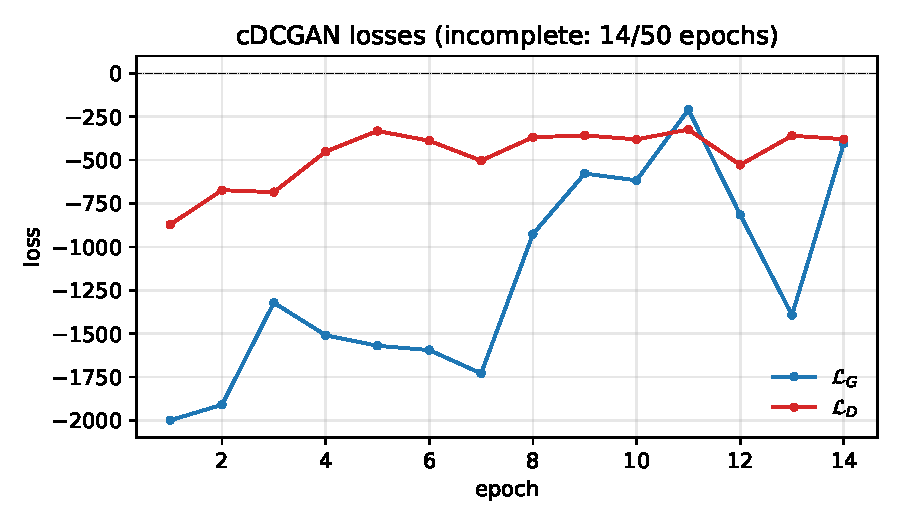
\includegraphics[width=0.7\textwidth]{../figures/cdcgan_loss.pdf}
  \caption{cDCGAN per-epoch generator and critic losses over the
           14 completed epochs.}
  \label{fig:cdcgan_loss}
\end{figure}

\subsubsection*{Game integration}
\label{sec:game}
We built a small \texttt{pygame} navigation game (\texttt{game/game.py}) in
which the player walks from a green start to a red goal across the generated
$128{\times}128$ terrain map; deep and shallow water are impassable and the
remaining four palette tiers map to per-cell movement-speed multipliers
$\{0.6, 1.0, 0.4, 0.2\}$. An A* solver computes the optimal traversal time on
the same speed grid and the in-game timer is graded against it.

The game accepts \texttt{--source perlin} (default; calls
\texttt{noise.create\_noise\_map} directly) or \texttt{--source gan
--preset preset\_NN}, in which case it loads an exported
\texttt{generator.npz} from \texttt{checkpoints/<preset>/}. The exported
weights are produced by \texttt{scripts/export\_generator.py};
\texttt{scripts/gan\_terrain.py} then performs the entire forward pass in
NumPy (BatchNorm, $3{\times}3$ convolutions via \texttt{im2col}, upsampling,
$\tanh$), so the game has no TensorFlow dependency. The raw $\tanh$ output is
mapped to $[0, 255]$, then each pixel is snapped to its
nearest-Euclidean-RGB palette entry; the same index lookup yields the discrete
speed map. All seven unconditional generators have been exported; the partial
cDCGAN checkpoint was not exported.

\begin{figure}[h]
  \centering
  \begin{subfigure}[t]{0.47\textwidth}\centering
    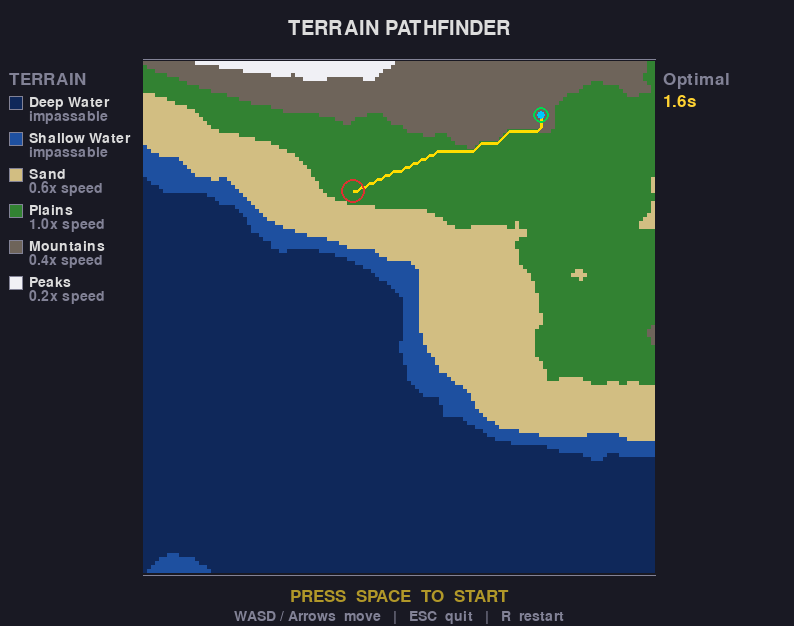
\includegraphics[width=\linewidth]{../screenshots/game_start.png}
    \caption{Perlin terrain at game start. The yellow overlay is the A*
             optimal path; the UI shows optimal traversal time of 1.6\,s
             before the player moves.}
  \end{subfigure}\hfill
  \begin{subfigure}[t]{0.47\textwidth}\centering
    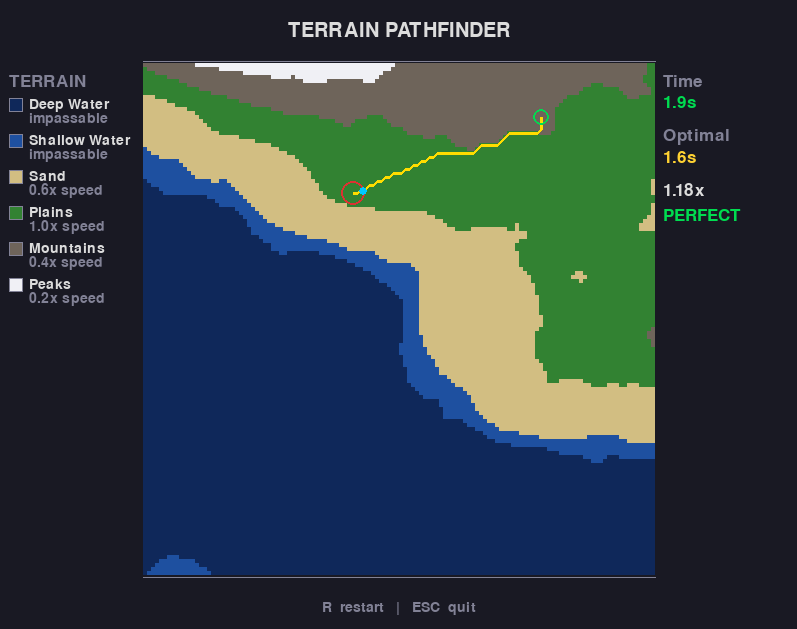
\includegraphics[width=\linewidth]{../screenshots/game_finish.png}
    \caption{Same Perlin terrain after goal reached. Actual time 1.9\,s
             (1.18$\times$ optimal); graded ``PERFECT''.}
  \end{subfigure}

  \vspace{0.6em}

  \begin{subfigure}[t]{0.47\textwidth}\centering
    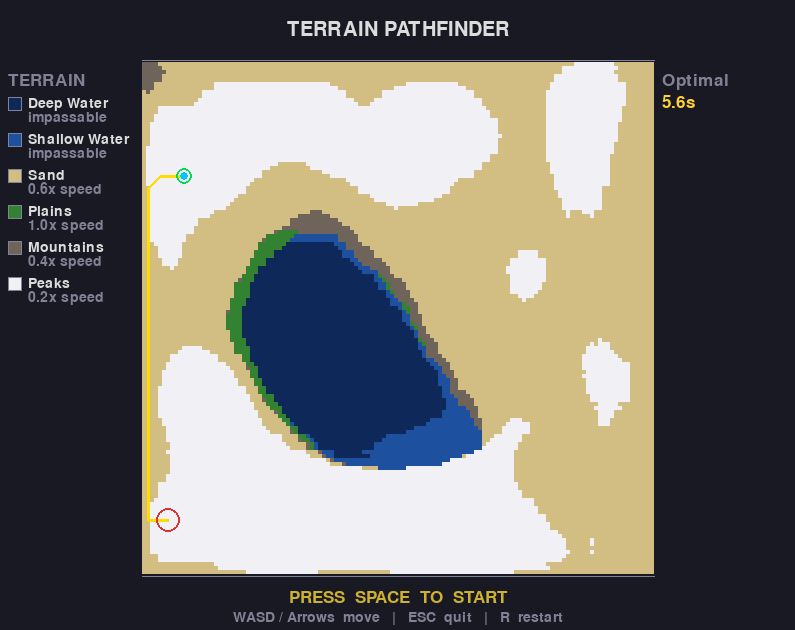
\includegraphics[width=\linewidth]{../screenshots/game_preset_01.png}
    \caption{GAN terrain (\texttt{--preset preset\_01}). Sand/peak mode
             collapse; A* optimal time 5.6\,s due to slow terrain.}
  \end{subfigure}\hfill
  \begin{subfigure}[t]{0.47\textwidth}\centering
    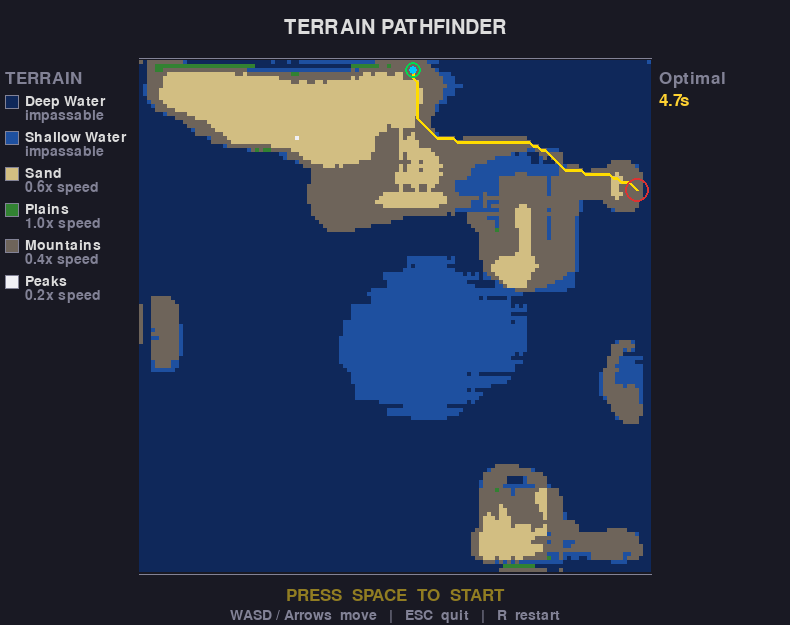
\includegraphics[width=\linewidth]{../screenshots/game_preset_03.png}
    \caption{GAN terrain (\texttt{--preset preset\_03}). Single oval water
             body; A* path (4.7\,s) circumnavigates the impassable water.}
  \end{subfigure}
  \caption{In-game screenshots. Top row: Perlin-noise source (default).
           Bottom row: GAN source. The terrain legend, A*~path, player
           position, and real-time score are rendered by
           \texttt{game/game.py}.}
  \label{fig:game_screenshots}
\end{figure}

% ─────────────────────────────────────────────────────────────────────────────
\subsection{Discussion and Comparison}
\label{sec:discussion}

\paragraph{Per-preset qualitative analysis.}
\begin{description}[leftmargin=1.5em, style=nextline, itemsep=2pt]
  \item[preset\_02, preset\_06] These two recover the macro-scale structure
    most convincingly. The generator produces plausible land/water boundaries
    with reasonable shape diversity across $\mathbf{z}$, and the dominant
    palette colors (deep navy water, light cream/sand) are present. Higher
    palette tiers (mountains, mountain tops) are not visibly recovered;
    transitions are smoothed rather than thresholded.
  \item[preset\_03, preset\_04] These show partial structure but a clear
    \emph{single-feature} mode: nearly every preset\_04 sample places one
    bright island near the center of a dark sea; preset\_03 places one
    elongated water body in a noisier yellow-green field. Within-grid
    diversity exists in shape and position but not in feature count, which is
    a textbook mode-collapse signature.
  \item[preset\_01, preset\_05, preset\_07] These collapsed most severely.
    The output is dominated by a single background color (yellow/cream for
    01 and 07; deep blue for 05) with at most one localized blob of contrast.
    The overall color distribution is qualitatively wrong relative to the
    training data: preset\_01 training samples are dominated by water and
    plains green, but the generator has settled on a sand-yellow background.
\end{description}

\paragraph{Why the discrete palette is hard.}
The Perlin-noise data has a piecewise-constant color field with sharp
boundaries at the six fixed thresholds. A $\tanh$-output convolutional
generator must learn six near-step-function responses in RGB space conditional
on the underlying smooth noise field it is implicitly synthesizing. With
$\mathrm{LReLU}$ activations and BatchNorm, gradient flow naturally favors
smooth output ramps; we observe exactly this -- the generator interpolates
between palette colors rather than thresholding them. Snap-to-palette
post-processing at inference time (Figure~\ref{fig:snapped}) closes most of
this gap visually.

\paragraph{Comparison with the real (Perlin-noise) distribution.}
The real Perlin-noise maps serve as the baseline; all quantitative metrics
compare generated distributions to the 200-image held-out test split.

\textit{FID.} FID (Table~\ref{tab:metrics}) ranges from 340 to 424.
These values are high by ImageNet-GAN standards, expected given the small
evaluation set (200 samples per side) and the mismatch between InceptionV3
features and synthetic terrain. The FID ranking does \emph{not} agree with
the qualitative assessment: preset\_07 achieves the lowest FID (340) despite
being visually collapsed, while the strongest visual generator (preset\_02)
has the highest FID (424). This reversal suggests the InceptionV3 embedding
is a poor proxy for the terrain structure we care about. The power-spectrum
and navigability metrics below are more informative.

\textit{Power-spectrum slope.} Real terrain images yield
$\beta \approx -2.5$ to $-2.6$, consistent with the $1/f^2$ power law of
layered Perlin noise. All seven generators produce steeper spectra
($\Delta\beta < 0$, range $-0.29$ to $-0.83$), meaning generated images
over-emphasize large-scale structure and suppress the mid- and
high-frequency detail present in the training data. preset\_07 deviates least
($\Delta\beta = -0.29$); preset\_04 deviates most ($\Delta\beta = -0.83$),
consistent with its strong single-feature mode collapse.
Figure~\ref{fig:psd} shows the mean radial power spectra for all seven presets.

\begin{figure}[h]
  \centering
  \begin{subfigure}[t]{0.32\textwidth}\centering
    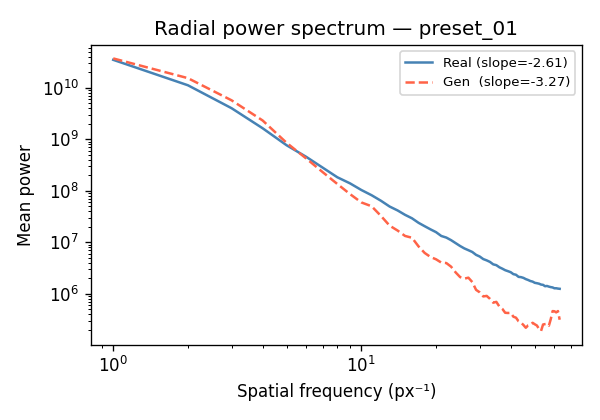
\includegraphics[width=\linewidth]{../results/psd_preset_01.png}
  \end{subfigure}\hfill
  \begin{subfigure}[t]{0.32\textwidth}\centering
    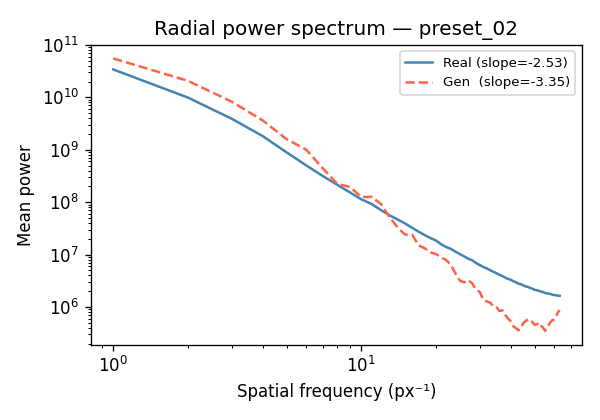
\includegraphics[width=\linewidth]{../results/psd_preset_02.png}
  \end{subfigure}\hfill
  \begin{subfigure}[t]{0.32\textwidth}\centering
    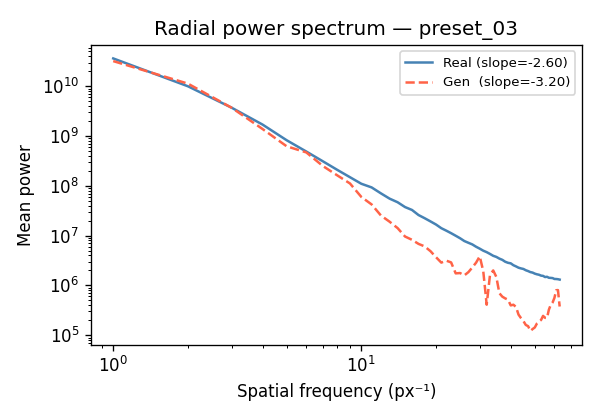
\includegraphics[width=\linewidth]{../results/psd_preset_03.png}
  \end{subfigure}

  \vspace{0.4em}

  \begin{subfigure}[t]{0.32\textwidth}\centering
    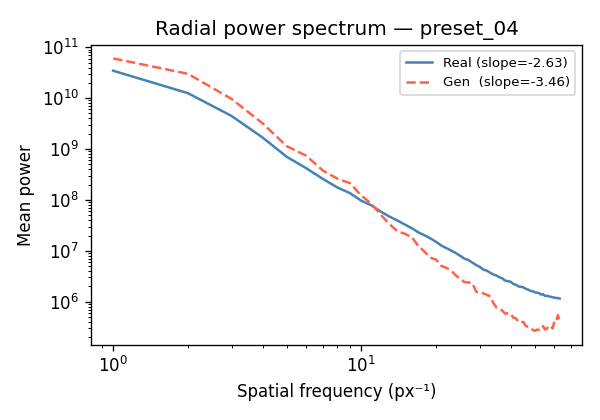
\includegraphics[width=\linewidth]{../results/psd_preset_04.png}
  \end{subfigure}\hfill
  \begin{subfigure}[t]{0.32\textwidth}\centering
    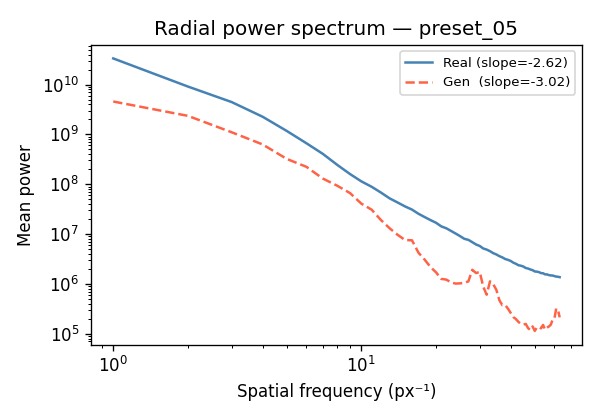
\includegraphics[width=\linewidth]{../results/psd_preset_05.png}
  \end{subfigure}\hfill
  \begin{subfigure}[t]{0.32\textwidth}\centering
    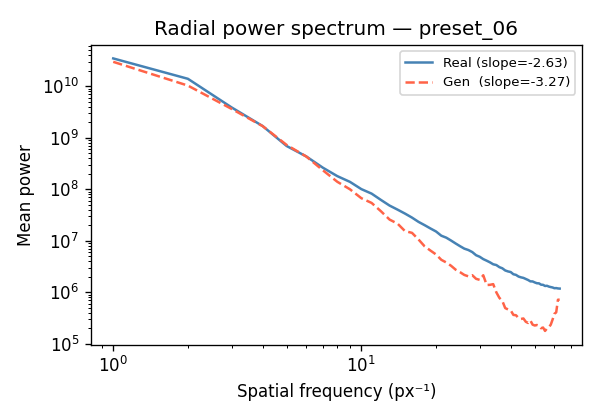
\includegraphics[width=\linewidth]{../results/psd_preset_06.png}
  \end{subfigure}

  \vspace{0.4em}

  \begin{subfigure}[t]{0.32\textwidth}\centering
    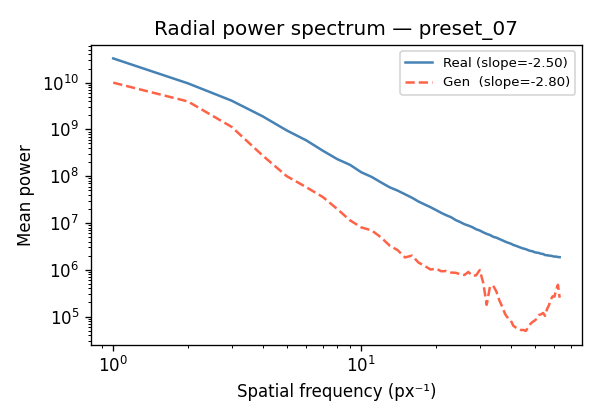
\includegraphics[width=\linewidth]{../results/psd_preset_07.png}
  \end{subfigure}
  \caption{Radially-averaged 2D power spectra (mean over 200 real and 200
           generated images per preset, log-log axes). Generated images have
           uniformly steeper slopes, reflecting the generator's tendency to
           produce large smooth blobs rather than the multi-scale detail of
           Perlin noise.}
  \label{fig:psd}
\end{figure}

\textit{Palette RMSE.} Real images score 0.0 by construction. Generated
palette RMSE ranges from 36.5 (preset\_03) to 64.1 (preset\_07), confirming
that all generators interpolate between palette colors rather than learning to
threshold them. Palette RMSE does not correlate strongly with FID: a
generator that collapses to one dominant palette color can achieve low RMSE
while producing poor spatial statistics.

\textit{Navigability.} Real images score tortuosity $\approx 1.27$--$1.30$
and reachable fraction $\approx 0.91$--$0.98$. Generated maps show uniformly
higher tortuosity (1.34--1.56) but more variable reachable fraction.
preset\_06 closely matches both real axes (tortuosity 1.45, reachable 0.98),
consistent with its strong visual quality. preset\_05 collapses to the lowest
reachable fraction (0.35): the generator produces a map dominated by
impassable water with one small island, leaving most passable area
disconnected. presets 03 and 04 similarly show low reachable fraction (0.63
and 0.60) due to single-feature collapse.

\paragraph{What worked.}
WGAN-GP trained stably for all eight runs; no run diverged or required
restart. The macro-scale spatial statistics are recovered for at least two
presets. End-to-end integration into the navigation game (NumPy inference,
snap-to-palette, A* solver, in-game scoring) works for all seven
generators.

\paragraph{What didn't.}
(i)~The discrete six-tier palette is not learned -- outputs interpolate
between colors rather than thresholding them.
(ii)~Three of seven generators show clear single-feature mode collapse.
(iii)~The cDCGAN did not finish training on CPU.
(iv)~FID correlates poorly with visual quality for this data; power-spectrum
slope and navigability are more interpretable signals.

\paragraph{Why CPU mattered.}
The same architecture on a single mid-range GPU would have completed all
seven unconditional runs in under an hour each (vs. 8--10\,h CPU) and the
cDCGAN in roughly 4--5\,h. The 50-epoch ceiling was a direct consequence of
CPU wall time; the lack of palette recovery and the mode collapse on three
presets are both partly attributable to undertraining.

% ─────────────────────────────────────────────────────────────────────────────
\section{Conclusion}
We trained seven WGAN-GP terrain generators on a synthetic Perlin-noise
dataset and analyzed their behavior across a deliberately heterogeneous
preset library. Training was stable but compute-limited; the resulting
samples reproduce the broad spatial statistics of the data on roughly half
the presets and exhibit single-feature mode collapse on the rest.
Quantitative evaluation (Section~\ref{sec:eval}) confirms these qualitative
findings: preset\_07 achieves the best FID (340) and smallest
power-spectrum deviation ($\Delta\beta = -0.29$), while the collapsed
presets (03, 04, 05) show reachable-area fractions well below the real
distribution (0.35--0.63 vs.\ 0.91--0.98). A planned conditional extension
reached only epoch 14 of 50 in the available CPU time. The trained generators
were successfully integrated into a real-time A* navigation game
(Section~\ref{sec:game}) via a NumPy-only forward pass with snap-to-palette
post-processing, demonstrating the end-to-end use case of the proposal.

\paragraph{Future work.}
The most productive next steps in roughly increasing scope are:
(1)~moving snap-to-palette (or a soft, differentiable approximation) into
the training loss to address the smooth-interpolation artifact at the source;
(2)~replacing BatchNorm in $G$ with LayerNorm or no-norm, which decouples
samples within a minibatch and removes the documented WGAN-GP /
BatchNorm-in-$G$ instability;
(3)~longer training of the cDCGAN on GPU, which is the natural home for the
``select terrain type at game-time'' use case;
(4)~a categorical-output reformulation -- predicting one of six palette
tiers per pixel via a softmax head and a cross-entropy auxiliary loss --
which would replace the regression-against-RGB problem with a much more
natural classification problem for this data.

% ─────────────────────────────────────────────────────────────────────────────
\bibliographystyle{plain}
\begin{thebibliography}{9}
\bibitem{gulrajani2017improved}
I.~Gulrajani, F.~Ahmed, M.~Arjovsky, V.~Dumoulin, A.~Courville.
\textit{Improved Training of Wasserstein GANs.}
NeurIPS 2017.

\bibitem{radford2016dcgan}
A.~Radford, L.~Metz, S.~Chintala.
\textit{Unsupervised Representation Learning with Deep Convolutional
Generative Adversarial Networks.}
ICLR 2016.
\end{thebibliography}

\vspace{1em}
\noindent\small\textit{Assistance from Claude AI.}

\end{document}
